\documentclass[draftclsnofoot,onecolumn,10pt,compsoc]{IEEEtran}
\usepackage[margin=0.75in]{geometry}
\usepackage{enumitem}
\usepackage{float}
\usepackage{caption}
\usepackage{url}
\usepackage{graphicx}
\graphicspath{ {./} }
\usepackage{titlesec}

% Set the size of the section and subsection headers
\titleformat*{\section}{\Large\bfseries\scshape}
\titleformat*{\subsection}{\large\bfseries}
\titleformat*{\subsubsection}{\normalsize\bfseries}

% Remove paragraph indent
\setlength\parindent{0pt}

% Better spacing for bibitems
\newlength{\bibitemsep}\setlength{\bibitemsep}{.2\baselineskip plus .05\baselineskip minus .05\baselineskip}
\newlength{\bibparskip}\setlength{\bibparskip}{0pt}
\let\oldthebibliography\thebibliography
\renewcommand\thebibliography[1]{%
  \oldthebibliography{#1}%
  \setlength{\parskip}{\bibitemsep}%
  \setlength{\itemsep}{\bibparskip}%
}

% Set single spacing
\usepackage{setspace}
\singlespacing

\begin{document}

\title{%
  Design Document \\[10pt]
  \Large Automate the Settings that Control a Million-Dollar Printing Press}
\author{\vspace{25pt}
\IEEEauthorblockN{Cole Jones \& Kuan-Yu Lai}\\
\IEEEauthorblockA{Group 62\\
CS 461 - Senior Software Engineering Project\\
November 23, 2019 - Fall Term}}

% make the title area
\maketitle

% Project abstract summarizing the entire document in 100-150 words.
\vspace{50pt}
\begin{abstract}
This document describes a year plan of the project that builds the assisting feature for the million-dollar printing press from HP. The goal of the project is to create a feature that can recommend the press settings of the giant press based on job inputs uploaded from the user. There are several components involved in building the feature: the rules engine, database, and website. This document describes the design viewpoint from different aspects for those components use in the project, such as what is the purpose of having this component and how does it interact with others components. It also contains the different technologies uses and the design schedule throughout the year.
\end{abstract}

\pagebreak
\tableofcontents

\bigskip
\listoffigures

% Project overview, description of stakeholders
\pagebreak
\section{Overview}
\subsection{Scope}
The objective of this project is to create a rules-based engine that takes an input object containing information about a print job and outputs a selection of settings used to control the printing press. The engine will run alongside existing internal tools, taking input from upstream pre-flighting and handing output downstream into the print job queue. The main components of the project will be the rules engine itself, a database to hold variables and constraints for the engine in addition to its outputs, and a web-based front-end with which the user will interact to provide job inputs.

\subsection{Purpose}
The purpose of this project is to simplify the process of selecting the optimal printing press settings for any given print job on any given press. The purpose of this document is to provide a detailed description of the design of each component of the project in addition to providing a clear path of development.

\subsection{Description of stakeholders}
Our clients are Mr. Pieter Van Zee and Mr. Ronald Tippetts from HP. They are both senior engineers with excellent experience with the printing presses. Their ultimate goal is for us to make a system for the printing press that only require a user to press a single button and then the machine will cover the rest. As the leader and user of the project, they provide feedback and suggestion to us based on our weekly research. At the same time, they are also researching on this topic as well, sharing their knowledge with us during the weekly meetings.

% Glossary of terms
\bigskip
\section{Glossary of Terms}
\begin{center}
    \begin{tabular}{|c|c|}
        \hline
        \textbf{Term} & \textbf{Description}\\
        \hline
        % Leaving this as an example of how the table should be set up
        Ruleset & A set of rules which the decision-making engine uses to generate optimal job settings.\\ & Includes information about best practices, optimal ink coverage\\
        \hline
        Rules Engine & A software system that executes one or more rules in a runtime production\\& environment. Rules take the form of true/false assertions, much like an if statement\\
        \hline
        Black Box & A system whose internal mechanism is usually hidden from or mysterious to the user. \\
        \hline
        API & A protocol that allows client communicate with the server easily\\
        \hline
        Redis & An open-source database that use in-memory data structure to store all of the data\\
        \hline
        Drools & A rules engine developed by Red Hat. Part of jBPM Workbench.\\
        \hline
    \end{tabular}
\end{center}

\bigskip
\section{Timeline}
 \vspace{-5mm}
\begin{figure}[h]
    \makebox[\textwidth][c]{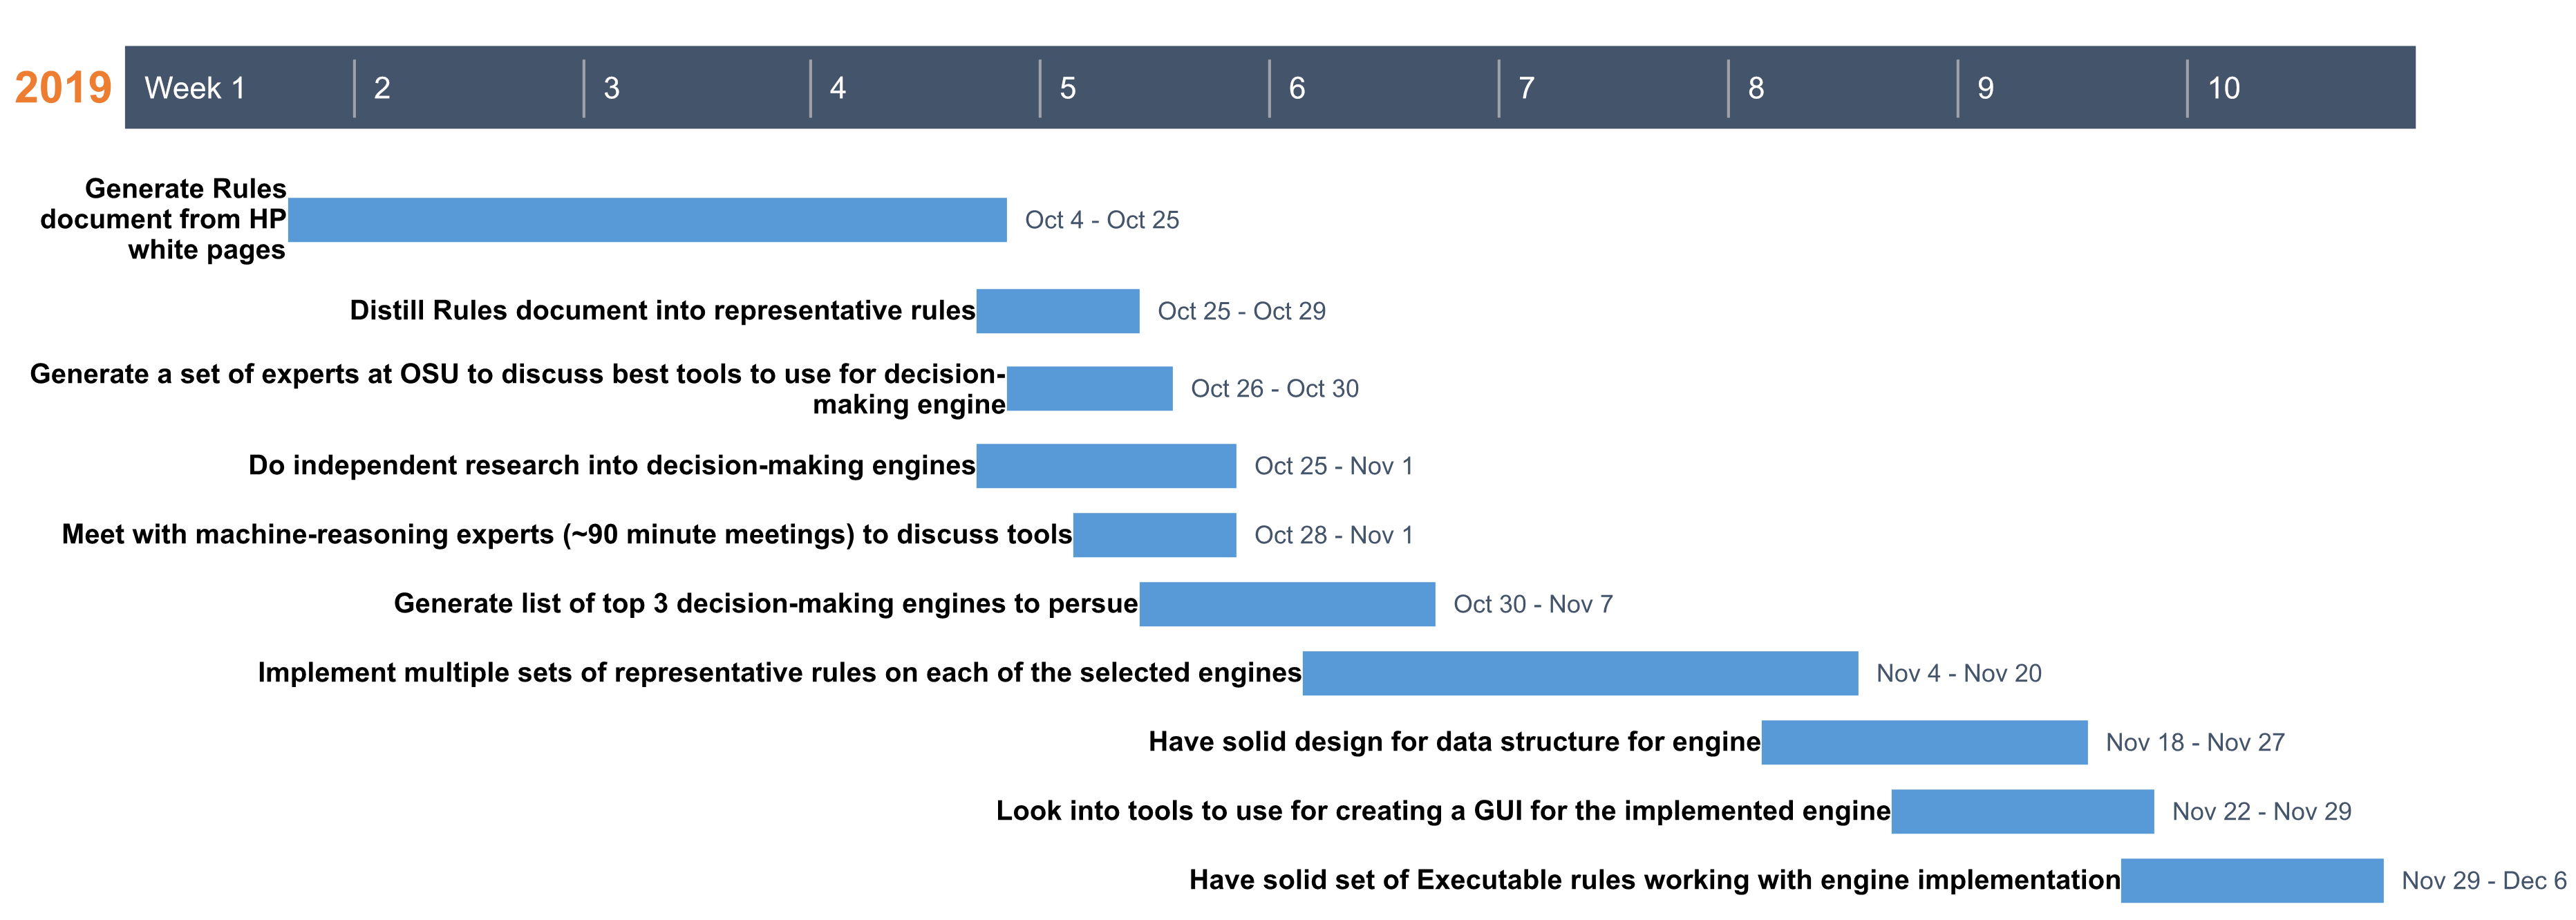
\includegraphics[width=1.05\textwidth]{Gantt}}
    \caption{Gantt Chart}
    \label{fig:1}
\end{figure}


% Design section 1 - Rules Engine
\pagebreak
\section{Rules Engine}
The rules engine will be handled by both Kuan-Yu and Cole equally, as it's the most integral part of the project and therefore requires the most attention.

\subsection{Description of Design}
The rules engine is the core of this project since it generates the ideal output for the user. One engine that has been considered is Drools, a Java-based business rules management system (BRMS) with both forward and backward chaining \cite{Drools}. It allows the user to generate their own ruleset, then fire as many rules as they deem necessary in any order. The engine uses an algorithm called the Phreak rule algorithm to evaluate the rules. Phreak is a faster and more efficient version of the Rete algorithm (a pattern matching algorithm invented in 1979), and it supports more evaluation methods \cite{Phreak}.\\[10pt]
Easy Rules has also been considered for use as it implements a similar rules-based engine, albeit in a much simpler way, foregoing the additional functionality of an engine like Drools for simplicity and portability \cite{Easy Rules}.

\subsection{Design Viewpoints}
\subsubsection{Context}
The rules engine will function as a sort of "black box." The user will provide input through either an API call or, more likely, the front-end website user interface. A series of scripts will manipulate the users inputs and call the engine's rules in a specific order to generate the output. The output will then be saved to the database and presented to the user.

\subsubsection{Composition}
The rules engine's functionality is defined in the following steps:
\begin{enumerate}
    \item Take user input passed from website/API call
    \item Use script to fire rules related to determining if the selected press is optimal
    \item Return to script and gather data generated from fired rule
    \item Continue firing rules to determine optimal settings
    \item When done firing rules, package output data and save to database
    \item Also return output data to front-end to present to the user
\end{enumerate}

\subsubsection{Dependency}
The rules engine depends on the existence of the database so that different rulesets can be fetched before runtime and engine outputs can be saved. Although it technically doesn't rely on the existence of the website, the site is the optimal method for interacting with the engine. The engine also depends on having an instance of the jBPM Workbench up and running, as the Drools engine was merged into the tool, and an instance of the KIE Execution Server to be able to use its built-in API for making calls to the engine.

\subsubsection{Interaction}
The rules engine will expose a REST API to the user so that calls may be made to fire its rules. This API will be called by the website to provide user input, so the user does not have to directly interact with the engine. Apart from passing rules and receiving output, the engine is a "black box." The user does not know what it going on inside of the engine. Outputs are also posted to the database by the control script.

\subsection{Design Rationale}
The reason why Drools/Easy Rules was chosen for the rules engine is because some technology akin to a decision tree was required, as opposed to the initial idea of using some type of machine learning. It was determined that the task was not suited to machine learning, and rule-based reasoning was settled on. Drools was chosen because it is a powerful open-source program with a large user base, and is currently in use by some groups at HP.

\subsection{Design Implementation}
The rules engine will be composed of a series of scripts, most likely written in a language like Python, that compiles user data into the correct format and sends it to the Drools engine by calling its built-in REST API. The script will be called from the website when the user submits their input data. It will most likely call the Drools engine multiple times, firing different rules to categorize the job data for future calls. After all of the rules have been called and the output is finalized, the script will make a call to post the data to the database, then will return the output to the website so it can be displayed to the user.


% Design section 2 - Database
%\bigskip
\pagebreak % Using a pagebreak for spacing while we write the document, might want to change it later
\section{Database}
Kuan-Yu will be responsible for this piece of the project, but others will help during the implementation as well. 

\subsection{Description of Design}
The purpose of the database is to store all of the data that is used in both the website and the rules engine. The database will categorize the data and provide quick access to the data while needed. 

\subsection{Design Viewpoints}
\subsubsection{Context}
The database provides important functionality to both the website and the rules engine. It will provide stable data access whenever needed by the rules engine or website. As a result, it is considered one of the most important pieces of this project. The data for the rules engine will be pre-stored in the database, but the data for the website will be based on the input of the user. 

\subsubsection{Composition}
The database functionality is defined in the following steps:\\
For interacting with the rules engine:
\begin{enumerate}
  \item Provide rules engine the rule set used to generate the result
  \item Provide rules engine the file uploaded from the user as the input
  \item Store the result generated from the rules engine
\end{enumerate}

For interacting with the website:
\begin{enumerate}
    \item Store the file provided from the user
    \item Store the setting set from the user
    \item Provide the recommended setting data generate from the rules engine
    \item Provide the data of existing tasks on the system
\end{enumerate}

\subsubsection{Dependency}
The database is dependent on both the website and the rules engine. Whenever they need a data-related service, it will be handled by the database. Therefore the input and output for the rules engine will be the recommended settings generated by the engine and the file uploaded from the user. For the website, the input and output will be the file uploaded from the user and the recommended settings as well as existing tasks.  

\subsubsection{Interaction}
The database does not directly interact with any other piece, rather the other pieces interact with the database. The control script running the rules engine will make a call to the database to fetch a ruleset or post its outputs. The website will make a call to the database to fetch all of the tables and update them if required, or to upload the user's input file.

\subsection{Design Rationale}
The reason why the database is a good choice to store the data is the categorize feature. It allows the user to categorize different kinds of data and find the relation of it. Therefore, it will increase the speed of searching and access to the data. In addition, there are different kinds of databases provided in the community and the majority of them are open-source, as a result, finding the right database can maximize the data access speed.

\subsection{Design Implementation}
The database will be implemented by a software called Redis \cite{redis}. The wide range of data types supported is the best fit for all of the data in this project. Furthermore, for the data which doesn't have any relation, Redis can access the specific data directly. The database will be held on the server and wait for the request all the time. Whenever the database receives an output request, it will search the data based on the request constrain and send back the data. If it receives an input request, it will store the data in the categorize space and assign a corresponding key to it.


% Design section 3 - Website
%\bigskip
\pagebreak % Using a pagebreak for spacing while we write the document, might want to change it later
\section{Website}
While anyone in the group is free to contribute to the website, the bulk of its creation will be handled by Cole.

\subsection{Description of Design}
The purpose of the website is to provide a front-end through which the user can interact with the tool. Both the rules engine and the database will be exposed to the website.

\subsection{Design Viewpoints}
\subsubsection{Context}
The website will provide a sort of "black box" view of the rules engine, allowing users to provide inputs about a print job and returning the outputs of its computation. By using a front-end, a minimal amount of the rules engine can be exposed to the user so as to minimize complexity. Users will also be able to view and manipulate the databases that store the variables that are used by the rules engine and the engine's previous outputs.

\subsubsection{Composition}
The website's functionality is defined in the following steps:\\
For interacting with the rules engine:
\begin{enumerate}
  \item Provide user a portal for entering print job inputs
  \item Make API call to rules engine, sending user input as body
  \item Receive output from rules engine
  \item Save output to database, also present to user
\end{enumerate}

For interacting with the database:
\begin{enumerate}
    \item Make API call to fetch the tables from the database
    \item Present the table to the user, allow them to edit entries
    \item Take the user's input and update the table in the database
\end{enumerate}

\subsubsection{Dependency}
The website depends on the existence of the rules engine, as well as its ability to take inputs and return outputs. It is also dependent on the existence on the database. The input will be information about the print job (collected via a form) like coverage and number of pages, and the output will be the result generated from the rules engine based on the input. 

\subsubsection{Interaction}
The website will provide three different modes for the user. First is the submission mode: in this mode the user will be able to submit the files they want to print. Second is the setting editing mode: this is for people to configure the setting of each individual printing task. Third is the submit mode: the user (most likely a manager or admin) can make sure the task is ready to submit.

\subsection{Design Rationale}
The reason why a website was chosen to create a front-end for used interaction, as opposed to, say, exposing only an API to the user, was to reduce the complexity of interacting with the rules engine and database. This front-end allows users to upload their job details via a form and to view the tables in the database without having to make database calls or API calls with curl. While the API is still available for users to call on their own, and can be used as an alternate method for invoking the rules engine, having a web application produces a sort of "black box" around the engine. This way, less responsibility is placed on the user.

\subsection{Design Implementation}
The website will be created using ReactJS as the main framework for structure, Bootstrap as the CSS framework for design, and React-Redux for managing application state. ReactJS is an open-source JavaScript library for creating user interfaces. It was launched by Facebook in early 2013 \cite{react-timeline}. It is optimized for applications where data on the page is changing rapidly. Bootstrap is the number one most popular open-source CSS framework that uses jQuery and JavaScript design templates to create user interfaces. It was created by Twitter in August 2011, and has since undergone three major rewrites to bring it up to version 4.0 \cite{Bootstrap}. React-Redux is a JavaScript library for managing application state, based paritally on Facebook's Flux \cite{Redux}.\\[10pt]
The design of the website is going to prioritize efficiency and usability. The user will be presented a simple and clean Bootstrap user interface that is easy to interact with. All of the API calls will be made using ReactJS to ensure speed when fetching database tables or making API calls. The website will be easy to use and efficient in its handling of data.


% Conclusion
\bigskip
\section{Conclusion}
In conclusion, this project consists of three major sections: the rules engine for evaluating inputs and producing optimal press settings as its output; a database to store all of the rulesets for the rules engine as well as all of its past outputs; a website to present a UI to the user and allow them to invoke the rules engine or view the contents of the database. The rules engine will be controlled by a script that determines the order in which to fire the rules, and the script will be invoked by the website when the user submits their inputs.\\[10pt]
The rules engine will be either Drools, an open-source business rules management system created by Red Hat, or Easy-Rules, a lightweight rules engine written in Java. The database will be constructed using Redis, an in-memory data structure project created by Redis Labs. The website will be a combination of ReactJS, a java framework created by Facebook, and Bootstrap, a CSS framework created by Twitter.


% Bibliography
\vspace{30pt}
\begin{thebibliography}{9}
\bibitem{Drools}
“Drools - Business Rules Management System (Java™, Open Source),” Drools. [Online]. Available: \url{https://drools.org/}. [Accessed: 23-Nov-2019].

\bibitem{Phreak}
“Chapter 5. Rule Algorithms Red Hat JBoss BPM Suite 6.2,” Red Hat Customer Portal. [Online]. Available: \url{access.redhat.com/documentation/en-us/red_hat_jboss_bpm_suite/6.2/html/development_guide/chap-rule_algorithms}. [Accessed: 23-Nov-2019].

\bibitem{Easy Rules}
M. B. Hassine, “j-easy/easy-rules,” GitHub, 18-Nov-2019. [Online]. Available: \url{https://github.com/j-easy/easy-rules}. [Accessed: 23-Nov-2019].

\bibitem{redis}
Redis.io. (2019). Redis. [online] Available: \url{https://redis.io/documentation} [Accessed 23-Nov-2019].

\bibitem{react-timeline}
A. Papp, “The History of React.js on a Timeline: @RisingStack,” RisingStack, 04-Apr-2018. [Online].\\
Available: \texttt{https://blog.risingstack.com/the-history-of-react-js-on-a-timeline/}. [Accessed: 23-Nov-2019].

\bibitem{Bootstrap}
M. Otto and J. Thornton, “About Bootstrap,” Bootstrap. [Online]. Available: \texttt{https://getbootstrap.com/docs/4.3/about/overview/}. [Accessed: 23-Nov-2019].

\bibitem{Redux}
“Redux · A Predictable State Container for JS Apps,” Redux. [Online]. Available: \texttt{https://redux.js.org/}. [Accessed: 07-Dec-2019].
\end{thebibliography}

\end{document}